\section{Experiments}
\label{sec:experiments}

\subsection{Implementation Details}

All experiments are run on a single GPU. The implementation uses
PyTorch~\citep{paszke2019pytorch}. Group convolution layers for the G-CNN are
implemented from scratch, without external equivariant-layer libraries.
The code repository is structured as follows: model definitions reside in
\texttt{models/}, data loading and preprocessing in \texttt{data/}, and the central
training loop in \texttt{train\_experiment.py}. All configurations are stored in
\texttt{config/} under Hydra's structured-config convention, with
\texttt{config/data/crc.yaml} specifying the NCT-CRC-HE-100K dataset parameters.

\subsection{Predicted Hypotheses}

Based on the theoretical motivation and related work \citep{veeling2018rotation}, we
anticipate the following patterns in the results:

\begin{enumerate}
  \item \textbf{G-CNN \(\geq\) CNN-Aug \(\geq\) CNN} in accuracy across all fractions.
    The architectural equivariance of the G-CNN provides a hard guarantee that
    augmentation can only approximate empirically.
  \item \textbf{Largest gap at small fractions.} The benefit of equivariance is
    expected to be most pronounced at the 5\%--20\% fractions, where the training
    set is too small for augmentation to cover the full orbit of each pattern.
  \item \textbf{Gap narrows at 100\%.} With sufficiently many samples, CNN-Aug may
    close most of the gap with the G-CNN, since it has seen each pattern in all
    orientations many times during training.
  \item \textbf{Rotationally isotropic classes (LYM, TUM) benefit most.}
    Circular tissue structures have the strongest rotational symmetry and should
    show the largest per-class improvement from equivariance.
\end{enumerate}

\subsection{Main Results}

\begin{table}[ht]
  \centering
  \caption{Test-set accuracy (\%) and macro-F1 (\%) on NCT-CRC-HE-100K across all
  training data fractions. \textbf{Bold}
  indicates the best result per fraction.
  }
  \label{tab:main_results}
  \renewcommand{\arraystretch}{1.2}
  \begin{tabular}{lcccccc}
    \toprule
    \multirow{2}{*}{Model} &
      \multicolumn{2}{c}{5\%} &
      \multicolumn{2}{c}{25\%} &
      \multicolumn{2}{c}{100\%} \\
    \cmidrule(lr){2-3}\cmidrule(lr){4-5}\cmidrule(lr){6-7}
    & Acc. & F1 & Acc. & F1 & Acc. & F1 \\
    \midrule
    CNN            & 0.56 & 0.51 & 0.67 & 0.64 & 0.83 & 0.77 \\
    CNN-Aug        & 0.75 & 0.66 & 0.76 & 0.72 & \textbf{0.89} & \textbf{0.84} \\
    G-CNN (\(p4m\))  & \textbf{0.78} & \textbf{0.71} & \textbf{0.8} & \textbf{0.73} & 0.86 & 0.8 \\
    \bottomrule
  \end{tabular}
\end{table}

\subsection{Data-Scaling Curves}

Figure~\ref{fig:scaling_curves} shows accuracy and macro-F1 as a function of the
training-set fraction for each of the three conditions. These curves are the primary
vehicle for assessing sample efficiency: a model with a stronger structural prior should
attain higher performance at small fractions, with the gap narrowing (or disappearing)
as the full dataset becomes available.

\begin{figure}[ht]
  \centering
  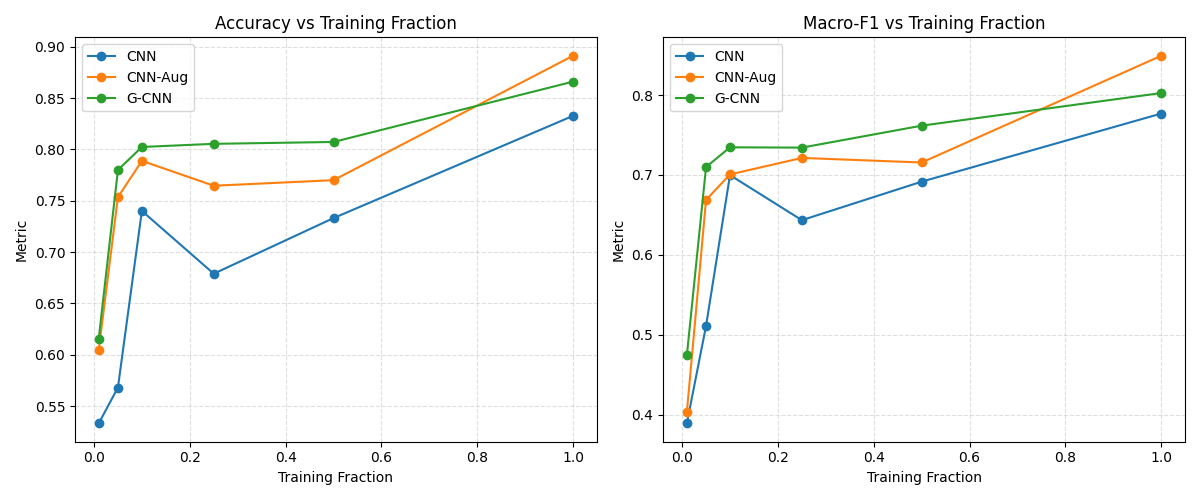
\includegraphics[width=0.9\linewidth]{figures/acc_f1_train_fraction.png}
  \caption{Test-set performance as a function of available labelled training data.}
  \label{fig:scaling_curves}
\end{figure}

As the experiments show, the G-CNN outperforms both other models, especially at low-data training regimes.
The G-CNN trained at 25\% of the data achieves very similar accuracy and F1 to the CNN-Aug trained at 100\%, 
demonstrating a significant boost in sample efficiency from the architectural equivariance. Although training
a normal CNN with data augmentation bridges the gap between the CNN and G-CNN, it does not fully close it, 
especially at the smallest fractions. This supports the hypothesis that architectural equivariance provides a 
stronger inductive bias than augmentation alone, particularly when training data is limited.

% \subsection{Per-Class Analysis}

% Table~\ref{tab:per_class} reports per-class F1 for each model at 100\% training data.
% Tissue classes with high rotational structure (e.g.\ LYM: lymphocyte clusters,
% TUM: glandular epithelium) are expected to benefit most from equivariance, as their
% appearance is approximately invariant under all 8 orientations in \(p4m\).

% "f1_macro": 0.6435295939445496,
%       "f1_class_0": 0.7622917890548706,
%       "f1_class_1": 0.9297475814819336,
%       "f1_class_2": 0.33503401279449463,
%       "f1_class_3": 0.8638073801994324,
%       "f1_class_4": 0.8416988253593445,
%       "f1_class_5": 0.449224591255188,
%       "f1_class_6": 0.6652806997299194,
%       "f1_class_7": 0.34456926584243774,
%       "f1_class_8": 0.6001121401786804

% \begin{table}[ht]
%   \centering
%   \caption{Per-class F1 (\%) at 100\% training data.}
%   \label{tab:per_class}
%   \renewcommand{\arraystretch}{1.2}
%   \begin{tabular}{lccc}
%     \toprule
%     Class & CNN & CNN-Aug & G-CNN (\(p4m\)) \\
%     \midrule
%     % ADI  & 0.90 & 0.99 & 0.97 \\
%     % BACK & 0.99 & 0.95 & 0.98 \\
%     % DEB  & 0.56 & 0.67 & 0.59 \\
%     % LYM  & 0.90 & 0.87 & 0.91 \\
%     % MUC  & 0.95 & 0.93 & 0.92 \\
%     % MUS  & 0.50 & 0.82 & 0.66 \\
%     % NORM & 0.75 & 0.85 & 0.86 \\
%     % STR  & 0.50 & 0.60 & 0.38 \\
%     % TUM  & 0.89 & 0.93 & 0.90 \\
%     ADI  & 0.76 & 0.99 & 0.97 \\
%     BACK & 0.92 & 0.95 & 0.98 \\
%     DEB  & 0.33 & 0.67 & 0.59 \\
%     LYM  & 0.86 & 0.87 & 0.91 \\
%     MUC  & 0.84 & 0.93 & 0.92 \\
%     MUS  & 0.44 & 0.82 & 0.66 \\
%     NORM & 0.66 & 0.85 & 0.86 \\
%     STR  & 0.34 & 0.60 & 0.38 \\
%     TUM  & 0.60 & 0.93 & 0.90 \\
%     \midrule
%     Macro & 0.64 & 0.84 & 0.80 \\
%     \bottomrule
%   \end{tabular}
% \end{table}

\